\subsection{Example: Calculating Parity of State}
\paragraph{Case 1: Calculate the parity of two nucleons in the $p_{3 /2}$ orbital} 
In the $p_{3 /2}$ orbital, we know $l = 1$. As all nucleons are fermions, the parity $π$ of the orbital is $(-1)^l = -1$.
\paragraph{Case 2: Calculate the parity of two nucleons in the $g_{9 /2}$ orbital}
In the $g_{9 /2}$ orbital, we know $l = 4$. As all nucleons are fermions, the parity $π$ of the orbital is $(-1)^l = 1$.

\subsection{Level Schemes \& Excited States}
\begin{itemize}
    \item Some nuclei have more excited states than others. This is regularly associated with even-$Z$ and even-$N$ nuclei in the interval $150 ≤ A ≤ 190$. 
    \item Comparing the level schemes of different nuclei : 
    \begin{figure}[h!]
    \centering
    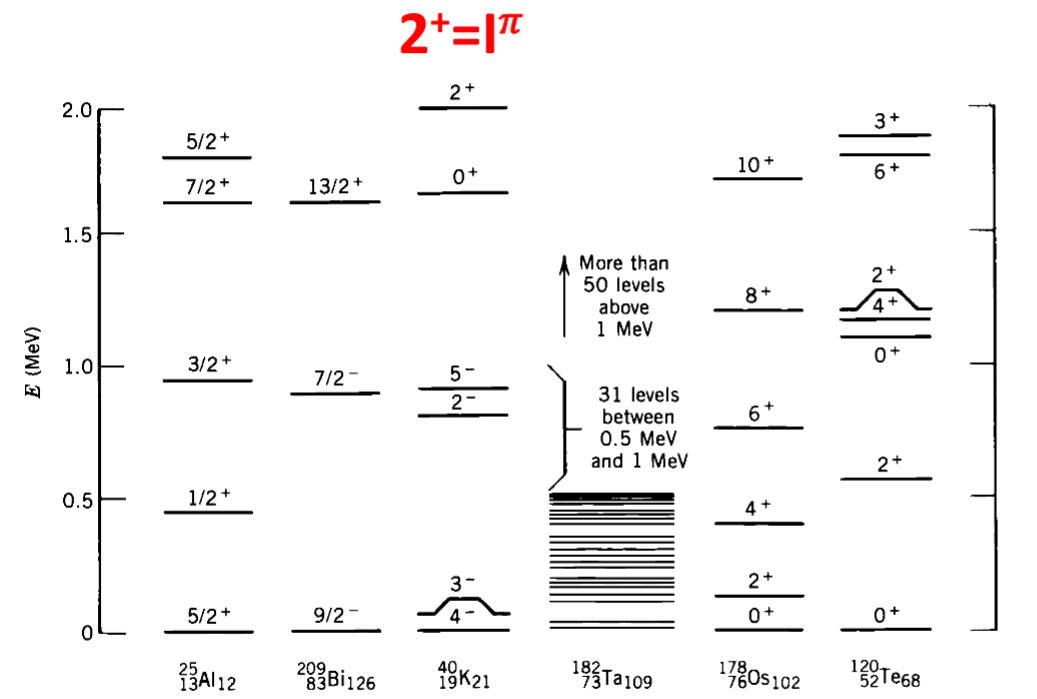
\includegraphics[width = .75\textwidth]{nuclei_excitation_levels_comparison.png}
    \caption{Some nuclei have more complex level schemes than others}
    \label{fig: nuclei_excitation_levels_comparison}
    \end{figure}
    
\end{itemize}


\section{Nuclear Force}
\begin{itemize}
    \item The strong force is very attractive at short distances. Even stronger than the Coulomb force. 
    \item Negligible at greater distances than 1-2 fm. 
    \item Some particles are immune, such as electrons. Electrons are 100,000 fm away from the nucleus.  
    \item The strong force becomes very repelling at distances smaller than 1 fm. 
    \item Nuclear force is nearly charge independent. We know this from experiments on excited states of \textit{mirror nuclei} (same $A$, but opposite $N$ and $Z$) as seen in \cref{fig: mirror_nuclei_excitation_levels_comparison}.
    \begin{figure}[h!]
    \centering
    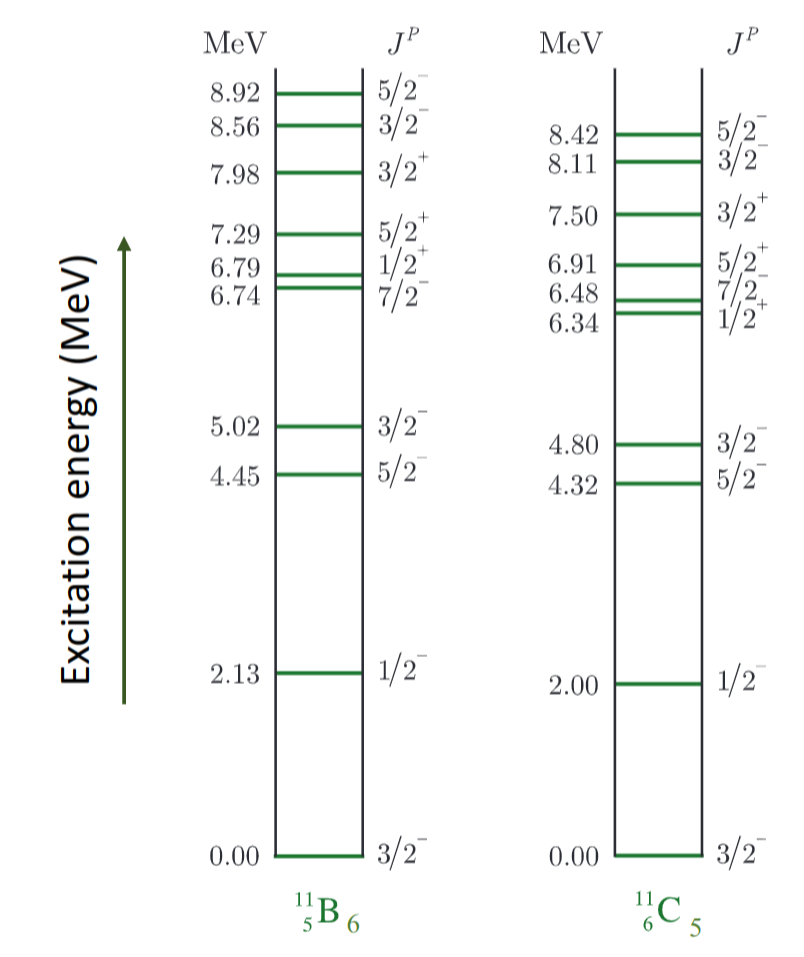
\includegraphics[width = .5\textwidth]{mirror_nuclei_excitation_levels_comparison.png}
    \caption{Comparison of the excitation levels of mirror nuclei. In this case we have $\displaystyle _{5}^{11}\text{B}_{6}$ and $\displaystyle _{6}^{11}\text{C}_{5}$}
    \label{fig: mirror_nuclei_excitation_levels_comparison}
    \end{figure} 
    
\end{itemize}

\subsection{Effects of the Short Range of the Strong Force}
\begin{itemize}
    \item When shooting alpha particles at a nucleus, the alpha particles are repelled by the Coulomb force if they do not have enough energy to get close enough to the nucleus. Then the strong force takes over and the alpha particles are attracted to the nucleus. This is why the Rutherford model does not work at lower energies. 
    \item The linear dependence on the binding energy per nucleon shows that the strong force is short range. If it were long range, each nucleon would attract all the others. Then the term in the binding energy as seen in the first therm of \cref{eq: semi_empirical_mass_formula}, would be quadratic and not linear $(α_vA)$
\end{itemize}

\subsection{Deuteron}
\begin{itemize}
    \item Consist of a proton and a neutron (nucleus of deuterium).
    \item To understand the structure of the atoms we would need to study its excited states. The problem is that deuteron is weakly bound and has no excited states.
\end{itemize}
\subsubsection{Deuteron Binding Energy}
There are multiple ways of calculating the binding energy of the deuteron. 
\begin{enumerate}
    \item \textbf{Mass spectroscopy}: Find the difference in mass between the deuteron and the proton and neutron.
    \begin{equation}
      B = \left( M\left(_{}^{1}\text{H}_{}\right) + m_n - m\left(_{}^{2}\text{H}_{}\right)\right)c^2 = 2.225 \text{ MeV}
    \end{equation} 
    \item \textbf{Nuclear reaction}: The gamma ray emitted when a neutron is captured by a proton is almost the binding energy. It has only energy, but can be converted to mass through $E = mc^2$.
    \begin{align}
    _{}^{1}\text{H}_{}& + n → \ce{_{}^{2}\text{H}_{}} + γ \\ 
    E_{γ} &≈ B = M_{\text{initial}} - M_{\text{final}} \\
    B &= \left( M\left(_{}^{1}\text{H}_{}\right) + m_n - M\left(_{}^{2}\text{H}_{}\right)\right)c^2 = 2.224 \text{ MeV}
    \end{align}
\end{enumerate}

\subsubsection{Nucleon-Nucleon Potential}
\begin{itemize}
    \item We assume that the potential between the nucleons is a finite square well with a potential depth of $-V_0$
    \item Solving for the Schrödinger equation for specific energy values and applying the boundary conditions we get the following results:
    \begin{align}
    &k_1 \cot \left(k_1 \vec{R}\right) = -k_2 \\
    &k_1 = \sqrt{\frac{2mE}{\hbar^2}} \quad k_2 = \sqrt{\frac{2m\left(V_0 + E\right)}{\hbar^2}}
    \end{align}
    \item The radius $R$ is now connected to the energy, and we know from scattering experiments that the radius is around 2.1 fm.
    \item The solution gives a potential of $V_0 = 35$ MeV. 
    \item The binding energy of the deuteron is just below the potential depth as seen in \cref{fig: deuteron_potential}.
    \begin{figure}[h!]
    \centering
    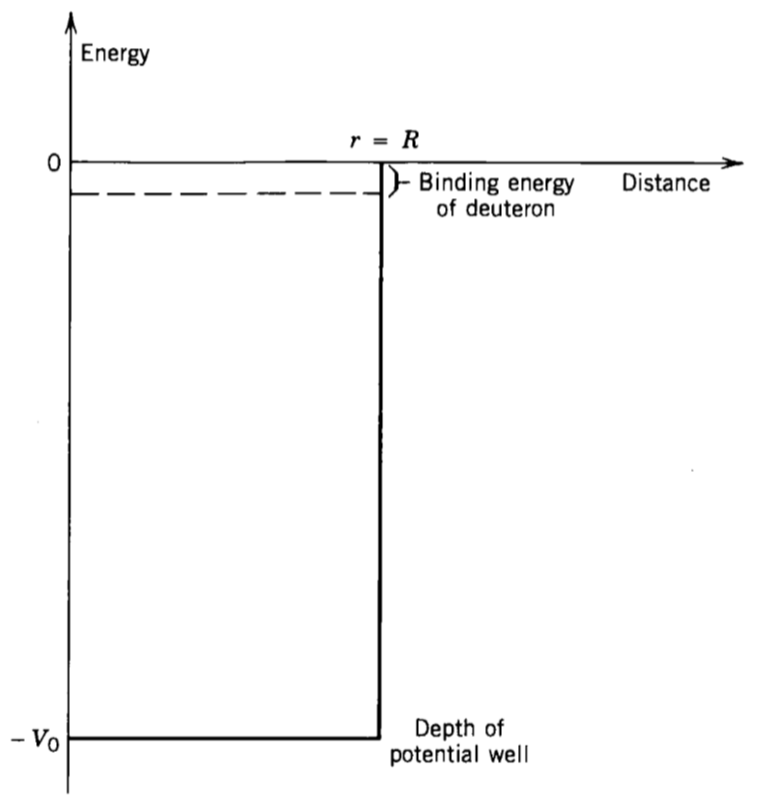
\includegraphics[width = .5\textwidth]{deuteron_potential.png}
    \caption{Square well potential for the deuteron. }
    \label{fig: deuteron_potential}
    \end{figure}
\end{itemize}

\subsubsection{Deuteron Spin and Parity}
\paragraph{Total Spin:}
\begin{equation}
  \vec{I} = \vec{S}_p + \vec{S}_n + \vec{l}
\end{equation}
\paragraph{Spin Configuration with $I = 1$}
\begin{enumerate}
    \item Aligning the spins gives $I = 1$ and $S = 1$ with $l = 0$. This is a positive parity state with $π = (-1)^{l} = 1$. We then get $I^{π}$ 
    \item Aligning the spins with gives $I = 3$
\end{enumerate}

\paragraph{Electric Quadrupole Moment}
The deuteron has a small non-zero electric quadrupole moment. This makes it so about 4\% of the time the deuteron is in an excited state with $l = 2$. 